\documentclass[UTF8]{beamer}

\usepackage{ctex}
\usepackage{setspace}
\usepackage{indentfirst}
\usepackage{ulem}
\usepackage{wasysym}
\usepackage{graphicx}

\usetheme{Szeged}
%\usecolortheme{seahorse}

\setlength{\parindent}{1.5em}
\setlength\parskip{.3\baselineskip}

\title{计算几何与字符串}

\author{h10}

\begin{document}

	\begin{frame}

		\maketitle

	\end{frame}

	\section{计算几何基础概念}

		\subsection{点,直线,向量}

			\begin{frame}{点}

			描述:在欧氏几何中,点是空间中只有位置,没有大小的图形,在二维欧氏空间中,一个点被表示为一组有序数对

			\end{frame}

			\begin{frame}{线}

			直线分为直线、射线与线段

			\pause

			一个问题,请问如何准确的定义点与直线

			\pause

			答:无法定义,试图去定义就会陷入重复定义、逆逻辑定义的深渊,点与直线作为原始概念的同时也具有原始概念的性质

			\end{frame}

			\begin{frame}{向量}

			在欧氏几何中,向量指具有大小和方向的量,它可以形象化地表示为带箭头的线段

			箭头所指:代表向量的方向;线段长度:代表向量的大小

			\end{frame}

			\begin{frame}{点积与叉积}

			在一个向量空间 $V$ 中,定义在 $V \times V$ 上的正定对称双线性形式函数即是 $V$ 的数量积(点积),而添加有一个数量积的向量空间即是内积空间

			$$
			a \cdot b = \sum _{i=1} ^k a_i b_i
			$$

			\pause

			向量积(叉积)可以定义为 $a \times b = a b \sin \theta$

			注意其中的 $a$ 与 $b$ 一般是一个三维向量,且向量积的结果是一个与 $a$ 和 $b$ 垂直的向量而不是标量

			\end{frame}

		\subsection{凸包}

			\begin{frame}{凸包的定义}

			广义定义:对于一个集合 $D$,$D$ 中任意有限个点的凸组合的全体称为 $D$ 的凸包

			数学定义:设 $S$ 为欧几里得空间 $R^n$ 的任意子集,包含 $S$ 的最小凸集称为 $S$ 的凸包,记为 $conv(S)$

			\end{frame}

			\begin{frame}{凸包求法}

			\href{Gift_wrapping_algorithm.gif}{\emph{\underline{Gift wrapping}}} : $O(|S|*|conv(S)|)$ 

			\href{Graham_scan.gif}{\emph{\underline{Graham scan}}} : $O(|S|*\log |S|)$

			\href{Quickhull.gif}{\emph{\underline{Quickhull}}} : $O(|conv(S)|*?)$

			\end{frame}

			\begin{frame}{旋转卡壳}

			\sout{这个算法名有 $16$ 种读法}

			\href{Rotating_calipers.gif}{\emph{\underline{Rotating calipers}}} : $O(|conv(S)|)$

			\end{frame}

			\begin{frame}{闵可夫斯基和}

			假设 $A$ 与 $B$ 都是一个点集,则有

			$$
			A + B = \{ a + b | a \in A, b \in B \}
			$$

			同理我们可以定义闵可夫斯基差

			$$
			A - B = \{ c | c + B \in A \}
			$$

			\pause

			关于闵可夫斯基和,有一个定理:

			$$
			|conv(A+B)| \le |conv(A)| + |conv(B)|
			$$

			\end{frame}

		\subsection{平面}

			\begin{frame}{平面图}

			在图论中,平面图是可以画在平面上并且使得不同的边可以互不交叠的图

			而如果一个图无论怎样都无法画在平面上,并使得不同的边互不交叠,那么这样的图不是平面图,或者称为非平面图

			完全图K5和完全二分图K3,3是最“小”的非平面图

			\end{frame}

			\begin{frame}{对偶图}

			在原平面图 $G$ 分割平面而得的每一个面置一个顶点(原平面图外部面也视为一个顶点),将相邻的面对应的顶点之间连一条边,这样构造出来的图叫做原平面图的对偶图,一般记为 $G^*$

			不难证明任何平面图的对偶图也是平面图,且平面连通图的对偶图的对偶图即为原图

			\end{frame}

			\begin{frame}{平面图转对偶图与点定位}

			\href{http://blog.miskcoo.com/2015/05/planar-graph-dual-and-point-locate}{\emph{\underline{平面图转对偶图}}}

			\href{https://en.wikipedia.org/wiki/Point_location}{\emph{\underline{点定位}}}

			\end{frame}

			\begin{frame}{半平面}

			欧氏平面被平面上一直线 $l$ 分割成两部分,其中每一部分都称做半平面,直线 $l$ 可以属于两半平面中的任一个

			半平面可以分为开半平面与闭半平面

			开半平面的代数定义如下:

			$a_1x_1 + a_2x_2 + ... + a_nx_n > b$

			闭半平面的代数定义如下:

			$a_1x_1 + a_2x_2 + ... + a_nx_n \ge b$

			\end{frame}

			\begin{frame}{半平面交}

			即多个半平面的相交部分

			求法与凸包类似,先把所有半平面按极角排序,再依次加入队列

			每次加入时判断队尾与队首的半平面是否有效,无效则删除直到有效为止

			\end{frame}

	\section{计算几何例题}

		\subsection{简单题}

			\begin{frame}{最近点对与最近圆对}

			题目很诚实,不想复述了

			\end{frame}

			\begin{frame}{最近点对与最近圆对}

			最近点对:分治,跨线点对暴力

			详见\url{https://www.cnblogs.com/Saurus/p/6119693.html}

			最近圆对:二分答案,扫描线

			详见\url{http://blog.sina.com.cn/s/blog_64675f540100o02x.html}

			\end{frame}

			\begin{frame}{bzoj2391}

			平面上有 $n$ 个膜法结点与 $m$ 只青蛙

			有 $q$ 次询问,每次从 $n$ 个膜法结点中按一定顺序选出一些构成膜法结界,膜法结界的形状是一个简单多边形(不自交但不一定凸的多边形),并将膜法结界内所有青蛙续一秒,求本次施法至少要准备多少秒时间

			每次询问保证不会有青蛙在被续的边缘试探而成为薛定谔的青蛙

			$n,m \le 1000, q \le 10000$

			\end{frame}

			\begin{frame}{bzoj2391}

			定义 $f[i][j]$ 为原点,膜法结点 $i$,膜法结点 $j$ 组成的三角形中的青蛙数,注意根据 $Cross(P[i],P[j])$ 的正负情况来决定 $f[i][j]$ 的正负

			于是询问可以线性了,现在考虑如何求 $f$

			先确定 $i$,定义其它所有膜法结点与青蛙的key值为 $i$ 到该点的极角大小

			把其它所有点按照原点与其连线的极角序排序,按顺序处理,遇到青蛙则加入平衡树,遇到膜法结点则询问

			\end{frame}

		\subsection{不简单题}

			\begin{frame}{CF \#433 Div.1 E}

			给你一个中心对称的凸多边形,将它分割成多个平行四边形

			$|S| \le 2000$

			\end{frame}

			\begin{frame}{51nod 1609}

			平面上有 $n$ 个点,且保证它们不全在一条直线上

			请找出一个 $1$ 到 $n$ 的排列 $p$,使得 $p_1$---$p_2$, $p_2$---$p_3$, ..., $p_{n-1}$---$p_n$, $p_n$---$p_1$ 这 $n$ 条线段两两不相交(可以在端点处相交)

			\end{frame}

			\begin{frame}{凸包最远点}

			众所周知,如果要求一个凸包的最远点对,旋转卡壳即可

			那么如果要对凸包上每一个点都要求出离它最远的点呢

			$n \le 100000$

			\end{frame}

			\begin{frame}{凸包最远点}

			答案其实是决策单调性DP...扔一下伪代码好了

			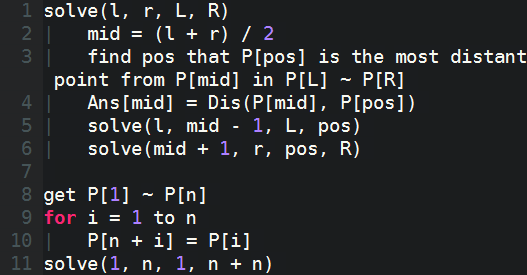
\includegraphics[height=4.5cm]{dp.png}

			\end{frame}

			\begin{frame}{uoj242}

			偷个懒,直接扔连接

			\href{http://uoj.ac/problem/242}{\emph{\underline{题面}}}

			\href{http://c-sunshine.blog.uoj.ac/blog/2026}{\emph{\underline{题解}}}

			\end{frame}

	\section{字符串基础}

		\subsection{匹配}

			\begin{frame}{Hash}

			Hash就是把任意长度的输入通过散列算法变换成固定长度的输出,该输出就是散列值

			这种转换是一种压缩映射,也就是,散列值的空间通常远小于输入的空间,不同的输入可能会散列成相同的输出,所以不可能从散列值来确定唯一的输入值

			\end{frame}

			\begin{frame}{Kmp}

			Kmp算法是一种改进的字符串匹配算法,由D.E.Knuth,J.H.Morris和V.R.Pratt同时发现,因此称之为Kmp算法

			Kmp算法的关键是利用匹配失败后的信息,尽量减少模式串与主串的匹配次数以达到快速匹配的目的

			具体实现就是实现一个next函数,函数本身包含了模式串的局部匹配信息,时间复杂度 $O(m+n)$

			\end{frame}

			\begin{frame}{AC Automaton}

			Aho-Corasick automaton,该算法在1975年产生于贝尔实验室,是著名的多模匹配算法

			简而言之,AC自动机就是Kmp算法在Trie树上的拓展,两者具有相似的时间复杂度

			\end{frame}

		\subsection{回文}

			\begin{frame}{Manacher}

			用于求以每个点为中心的最长回文串长度

			\end{frame}

			\begin{frame}{Palindromic Tree}

			用于记录全文所有本质不同的字串,并以它们为点建立一颗回文树

			\end{frame}

		\subsection{后缀}

			\begin{frame}{Suffix Array}

			在字符串处理当中,后缀树和后缀数组都是非常有力的工具,其中后缀数组是后缀树的一个非常精巧的替代品,可以节省许多空间

			主体部分就是对所有后缀按字典序大小排序,可以用来快速求两个后缀最长公共前缀等

			\end{frame}

			\begin{frame}{Suffix Automaton}

			亦是经典后缀处理算法之一,很多情况下可以用Suffix Array代替,但是代码简短

			不过Suffix Automaton的形态比较抽象

			\end{frame}

	\section{字符串例题}

		\subsection{简单题}

			\begin{frame}{bzoj3160}

			给定一个由 'a' 和 'b' 构成的字符串,求有多少个子序列满足

			1. 位置和字符都关于某条对称轴对称

			2. 不能是连续的一段

			$n \le 100000$

			\end{frame}

			\begin{frame}{bzoj3160}

			首先像Manacher算法一样的向字符串里插 \#

			考虑先求出总回文子序列的个数,然后减掉连续的,连续的就是回文子串,用Manacher算法可以 $O(n)$ 求解

			令 $f[i]$ 表示以 $i$ 为中心的对称字符对数量,那么对于每个中心 $i$ 我们有 $2^{f[i]}-1$ 种方案

			发现对 $f[i]$ 有贡献的一对字符在原字符串中的位置之和一定是 $i$

			FFT一下就好了

			\end{frame}

			\begin{frame}{bzoj4310}

			定义膜力串为一个字符串中字典序最大的子串

			给定一个字符串,请把它分成不超过 $k$ 个子串,并使这 $k$ 个子串中最大的膜力串尽可能小

			输出这个膜力串

			$k \le n \le 100000$

			\end{frame}

			\begin{frame}{bzoj4310}

			一共也就 $n^2$ 个子串,SA排序,二分答案

			从后往前贪心,记录当前右端点,左端点一路扫,如果当前子串大于二分的答案就分割

			\end{frame}

		\subsection{不简单题}

			\begin{frame}{bzoj2553}

			给定 $n$ 个膜法字符串 $T_1, T_2, ..., T_n$,对于一个字符串,如果把这个字符串划分为几个部分,如果某个部分正好是某一种膜法字符串,那么这个部分是有膜力的,并定义这个划分的膜力值为有膜力的部分的个数

			定义一个字符串的最佳划分为膜力值最大的划分,求长度为 $len$ 的字符串的最佳划分的膜力值的期望值

			$n \le 5, len \le 10^9, 0 < |T| \le 15$

			\end{frame}

			\begin{frame}{bzoj2553}

			看范围知算法:矩阵乘法

			对所有模式串建立AC Automaton

			令 $f[i][j][k]$ 表示从结点 $i$ 走 $k$ 步到结点 $j$ 的概率

			则 $f[i][j][k] = \sum _{p=1}^{size} f[i][p][k/2] * f[p][j][k-k/2]$

			对于任意 $i,j$,$f[i][j][1]$ 都是已知的,但是对于每个单词的结尾结点,要重新构造它的连边

			同时,为了统计答案,新开一个点,编号为 $size+1$,每个单词的结尾结点向它连边,边权为 $1$

			于是最后的 $f[0][size+1][len+1]$ 就是答案

			\end{frame}

			\begin{frame}{CC TASUFFIX}

			设数组 $A[i]=i$,大小为 $n$,对其进行 $m$ 次操作

			有两种操作:

			1. 把某一段提到开头

			2. 区间翻转

			操作完后问你后缀数组为 $A$ 的字符串 $S$ 有多少种可能。

			$S$ 的限制是字符串中出现的都是正整数,且最大元素等于不同的元素个数

			$n \le 10^9, m \le 10^5$

			\end{frame}

			\begin{frame}{CC TASUFFIX}

			我们来考虑一下题意:$suf[A_i,n] < suf[A_{i+1},n]$

			考虑到 $S$ 的限制,则一定有 $S[A_i] \le S[A_{i+1}]$

			当上式取小于号时,一定可行,现在主要是要看能不能取等于号

			发现等于号取到的条件就是 $suf[A_i+1,n] < suf[A_{i+1}]+1,n]$

			\end{frame}

			\begin{frame}{CC TASUFFIX}

			用Splay来得到最终的 $A$ 数组,其形式必定是:

			$[x_1,y_1], [x_2,y_2], ..., [x_k,y_k]$

			也就是一段段连续的区间

			我们发现当 $A_i, A_{i+1}$ 不在区间边界上的时候是一定可以满足取等的条件的,因此只需要考虑边界上是否满足条件即可,这个也很容易

			最后的答案就是 $2^p$,其中 $p$ 为可以取等的位置数

			\end{frame}

\end{document}

